\chapter{Cross Domain Learning For Online Advertisement}
\label{chapterlabel5}
\section{Domain Adaptation and Transfer Learning}
Traditional supervised learning is relied on the assumption that the distribution of training and test instances are similar. However, it is rare in real life that the distributions among datasets are unchanged. As discussed in \cite{facebook2015}, many proposed machine learning algorithms and models can be only used under the assumption that the training and test datasets are derived from the same distribution and with same feature space, when the distribution changes, new data needs to be collected and new model needs to be rebuilt. For the industry of online advertisement, it is expensive time-consuming to rebuild the model, in this case, transfer learning is needed which can borrow the knowledge learned from previous advertisement campaigns and apply to new campaigns to increase the efficiency for CTR prediction and decrease the cost for training new model. Although now directly related but similar to the research in \cite{pan2008transfer}, the behaviors of users among different campaigns are volatile and unpredictable, in traditional statistical machine learning problem, it is based on the ideal assumption that the model learned will not affect the real world, independent and identically distributed samples on different campaigns ensures the generalization. However when it comes to the real-world online advertisement industry, after the model is introduced into production, the users behavior will be affected, and also the distribution of the data. In brief, the changeable user behaviors among online advertisement campaigns determines that static statistical model is not suitable for dynamic online advertisement CTR prediction, \textit{transfer learning} is desirable which can save significant time and effort. 


\begin{figure}[t]
\centering
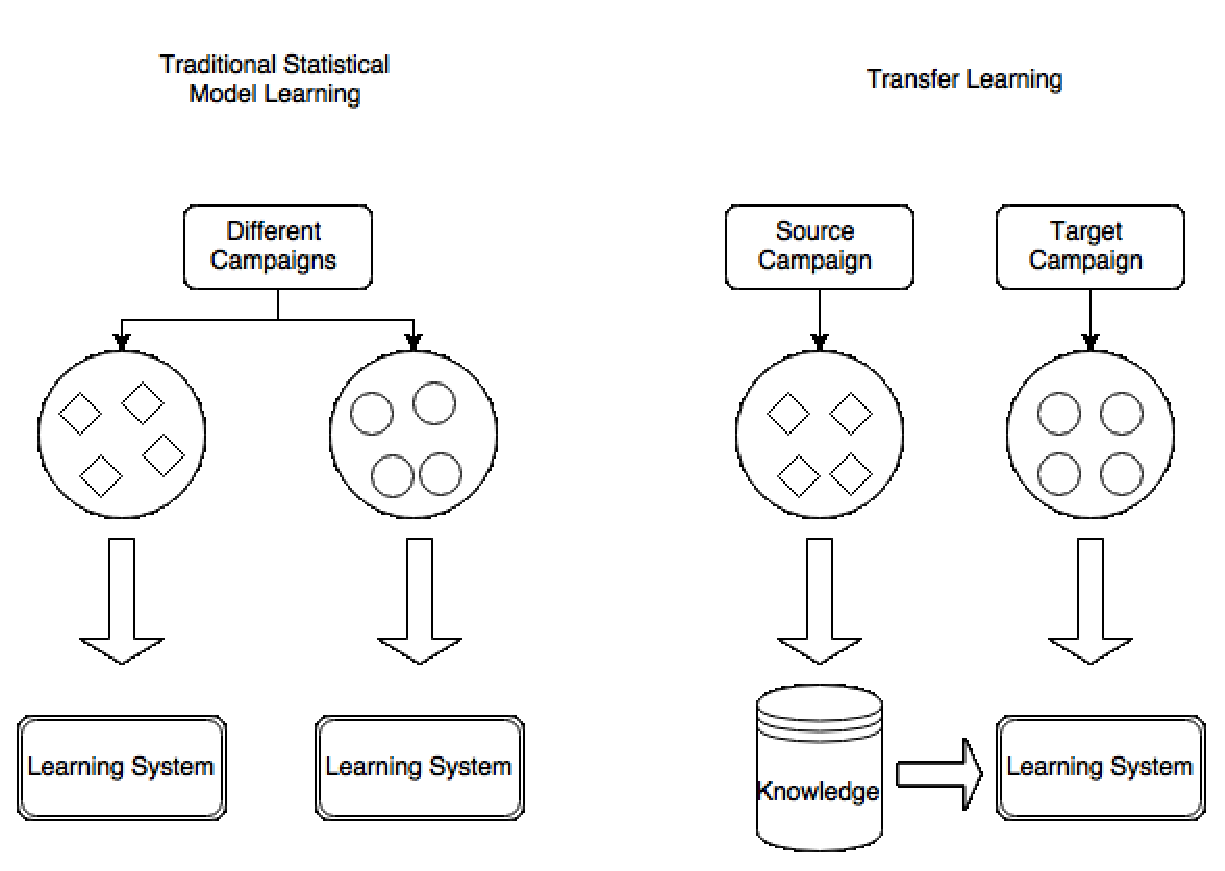
\includegraphics[width=\columnwidth]{transferlearning.eps}
\caption{Different Learning system between traditional machine learning and transfer learning}
\label{fig:transfer}
\end{figure}

At first, using the definitions in \cite{pan2010survey}, we specify \textit{domain} \textit{D} as each campaign's impressions raw data, and \textit{task} \textit{T} as the learning system of the model, in which, \(D = \{X,P(X)\}\), also  \(D = \{Y,P(Y|X)\}\). \(X = \{x_1,x_2, ..., x_n\}\) in which \(x_i\) is one impression in the campaign, and \(Y = \{y_1,y_2, ..., y_n\}\) is the label for each impression, namely whether in this impression the click occurs. The training data is composed of the pairs of \(\{x_i,y_i\}\) which can be used to train the model, and the conditional distribution \(P(Y|X)\). We define \textit{source domain} as the old campaign and \textit{target domain} as the new campaign, then \(X_s\) will be the feature space of source domain and \(P(X_s)\) is the marginal probability distribution of the feature space of source domain, similar, \(X_t\) will be the feature space of target domain and \(P(X_t)\) is the marginal probability distribution of the feature space of target domain. \(Y_s\) is the class label of the features in source domain and \(Y_t\) will be the corresponding label for target domain. By considering the relation between source domain and target domain, as well as source task and target task, the model learning problem can be classified as follows in the scope of online advertisement. 

\begin{enumerate}
\item if \(D_s = D_t\) and \(T_s = T_t\), this is a traditional machine learning problem. For example, the source and target advertisement campaigns follow the same distribution, and their learning tasks are the same, which are to predict the CTR based on the feature spaces. 

\item if  \(D_s \neq D_t\) and \(T_s = T_t\), which means the source and target domains are distinct but with the same tasks. The problem is also known as \textit{domain adaptation} \cite{arnold2007comparative} since the two domains are different in the marginal probability distribution but same for tasks. This situation can be further classified into two types:
    \begin{itemize}
    \item  \(X_s \neq X_t\), which means the feature spaces of the two domains are different with each other, for example, one domain of an advertisement campaign  \textit{International e-commerce} and the other is from \textit{ Software} as shown in \cite{zhang2014real}, if the impressions of the two domains are encoded into binary feature, surely there will be small overlap between the two feature spaces and the feature spaces will be largely different.
    \item \(P(X_s) \neq P(x_t) \), which means the probability distributions of the two advertisement campaigns are different, so they are from different fields, with different themes. 
    
    \end{itemize}
\item if  \(D_s = D_t\) and \(T_s \neq T_t\), it can also be classified into two types:
     \begin{itemize}
    \item  \(Y_s \neq Y_t\), this means the label spaces are different for two domains, as an example for online advertisement, the label in one domain could be click/non-click, which is dichotomic, but in the other domain the labels can be winning price, which is continuous.
    \item \(P(Y_s|X_s) \neq P(Y_t|X_t) \), this means the conditional probability distributions of the label on feature spaces are different for two domains, one example can be due to the existence of online robots, for one campaign all the impressions are randomly clicked or seen by programs, but the other campaign successfully prevent themselves from the robots so all clicks are effective and valid which simulates the human behaviors in the real world.  
  \end{itemize}
\end{enumerate}

In this paper, we will focus on transductive transfer learning, or \textit{domain adaptation}, since our learning task is obvious, which is CTR prediction, and we assumes that the robots are rare in the campaign, so the conditional probability are similar between the two campaigns, since the similar human behaviors will lead to similar advertisement clicking actions. 

As discussed above, domain is composed of feature space and feature probability distribution. In this paper, since our goal is to compare the performance of binary feature and counting feature, so we will represent the feature space and feature probability distribution of source and target domain in Table~\ref{tab:domainadapt}.

\begin{table}[t]
\begin{tabular}{ c | l | l }
Feature Types & Feature Space & Feature Distribution \\
\hline \hline
Binary Feature & Different & Different  \\
Counting Feature & Same & Different
\end{tabular}
\caption{Source and Target domain comparison for Binary and Counting Features}
\label{tab:domainadapt}
\end{table}

To clarify, for binary feature, suppose in the user dataset of online advertisement there is a categorical feature \textit{nationality}, with the value \textit{China}, \textit{Uk}, \textit{USA}, etc. It is not surprisingly that the original field space will be blew up to hundreds of features which is the number of countries in the world, without pre-processing, we even cannot distinguish \textit{Uk} from \textit{Great Britain}, which makes astronomical number of features with the increasing of new impressions. Microsoft claims that they have hundreds of millions features \cite{graepel2010web} for each training dataset, as we are already in the age of big data online advertisement, we can expect that the data volume will increase to the magnitude of hundred billion with hundred billion sparse discrete features. Even for our experiment, millions of features will arise from the dataset when the number of impressions reach 1 million. Therefore, the feature spaces are always distinct between the old campaigns and new campaigns. 









\section{Advertisement Campaign Datasets Shift}

\section{Cross-Dataset Generalization}

